\begin{frame}{AES T-Table Attacks with Flush+Reload on Allwinner D1 RISC-V ASIC}{\href{https://github.com/cispa/Security-RISC/blob/main/aes_example/fr/spy.cpp}{PoC} by Lukas Gerlach CISPA Helmholtz Center for Information Security }
    \begin{columns}
        \begin{column}{0.67\textwidth}
            \begin{itemize}
                \item AES uses S-boxes based on GF(256).
                \item The usage of these fields is \href{https://cr.yp.to/antiforgery/cachetiming-20041111.pdf}{\color{pink} not constant time}. 
                \item Implementations use 4 tables, each is 256 4-byte words.
                \item In OpenSSL-1.0.1e, table lookups are based on 
            \end{itemize}
            \begin{equation*}
                        T_j\left[p_i \oplus k_i\right] \hspace{1cm} j = i\ \%\ 4
            \end{equation*}
            So, in our attack on AES128, we will
            \begin{enumerate}
                \item Map libcrypto.so in attacker and victim processes
                \item Flush the data cache
                \item Trigger encryptions with a known plaintext value for $p_i$
                \item Measure access times for the S-box values to leak key bits
                \item Repeat 2-4 with for $i\ \in\ \left[0,\ 1,\ 2...\ 16\right] $
            \end{enumerate}
        \end{column}
        \begin{column}{0.33\textwidth}      
            \begin{figure}
                \centering
                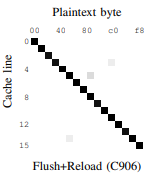
\includegraphics{images/flush_reload.png}
                \caption{Plaintext versus cache line access with a null key ($k_i = 0$)}
                \label{fig:flush-reload}
            \end{figure}
        \end{column}
    \end{columns}
    \note{
        \begin{itemize}
            \item We can recover the uppermost nibble of every byte, exponentially reducing the keyspace.
            \item The demo uses an instruction similar to the broken x86 clflush instruction, which allows cache maintenance in userspace. This is an instruction outside the RISC-V specification called \textit{dcache.civa}. 
            \item Flushing the data cache of the AES T-Tables also flushes it in the victim process as well. This is because the OS will map the two virtual addresses to the same physical address.
            \item This attack can be remedied by not exposing cache maintenance instructions to userspace processes.
            \item The hardware used here can be purchased cheaply off of eBay; most embedded SoCs do not have the means to issue patches to hardware attacks.
            \item In practice, this vulnerability is most practical for reverse engineering purposes, specifically for analyzing coprocessors with shared memory (such as the Wi-Fi chipset).
        \end{itemize}
    }
\end{frame}